% Supplementary material for "Beautified Is Not Forged" (moved from main.tex on 2026-09-29).
\documentclass[onecolumn]{IEEEtran}
\usepackage{fontspec}
\setmainfont{texgyretermes}[Extension=.otf,UprightFont=*-regular,BoldFont=*-bold,ItalicFont=*-italic,BoldItalicFont=*-bolditalic]
\usepackage{amsmath,amssymb}
\usepackage{graphicx}
\usepackage{booktabs}
\usepackage{adjustbox}
\usepackage{xcolor}
\usepackage[hidelinks]{hyperref}
\graphicspath{{figs/}}
\newcommand{\ours}{\textsc{Ours}}
\renewcommand{\thesection}{S\arabic{section}}
\renewcommand{\thetable}{S\arabic{table}}
\renewcommand{\thefigure}{S\arabic{figure}}
\begin{document}
\title{Beautified Is Not Forged: Supplementary Material}
\maketitle

\section{Figures and details moved from the main paper}
\begin{figure}[h]
\centering
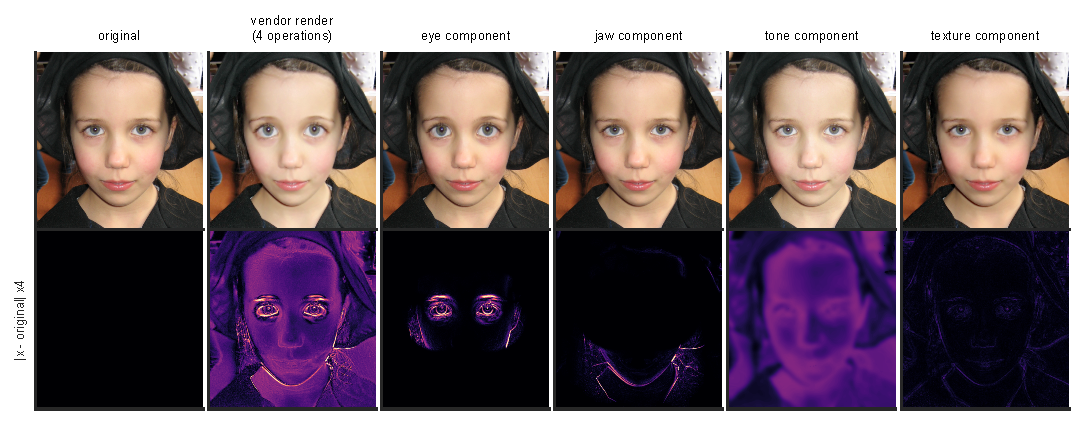
\includegraphics[width=0.9\linewidth]{fig_decomp}
\caption{Splitting a four-operation Tencent render into single-operation components in the original's geometry. Bottom:
absolute difference to the original, $\times$4. Eye and contour components are the render's optical flow restricted to
the eye regions and to the rest of the face; tone and texture components are the low- and high-pass parts of the
photometric residual. The four parts recompose the render.}
\end{figure}
\begin{figure}[h]
\centering
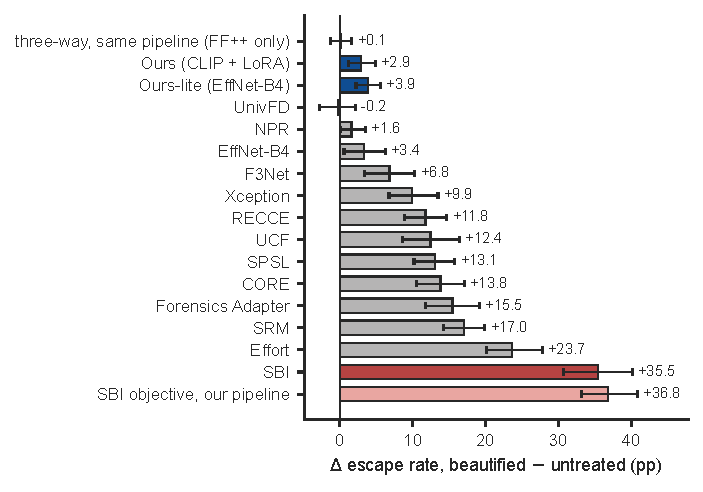
\includegraphics[width=0.5\linewidth]{fig_escape}
\caption{Celeb-DF-B: change in the share of deepfake frames called real when the same videos are beautified, with 95\%
video-cluster intervals. Binary detectors at 5\% FPR on untreated genuine frames; three-way models at their native rule.}
\end{figure}
\begin{figure}[h]
\centering
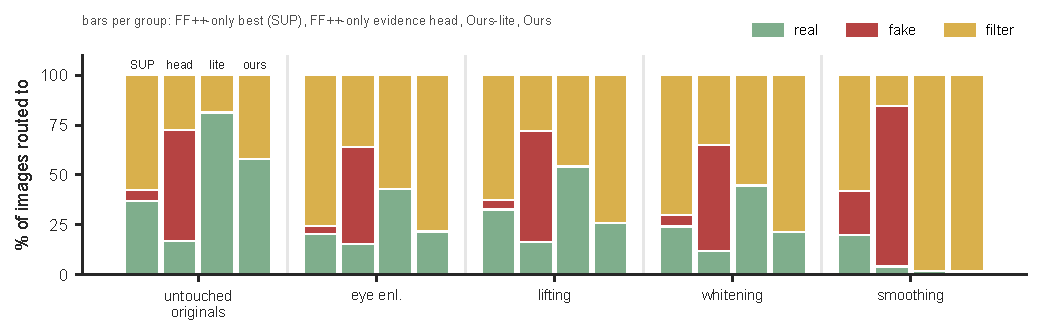
\includegraphics[width=0.9\linewidth]{fig_alibars}
\caption{Where the unseen service's retouched faces go (levels pooled): share routed to real, fake and filter for the best
FF++-only three-way model, the FF++-only evidence-head model, \ours{}-lite and \ours{}.}
\end{figure}
\begin{figure}[h]
\centering
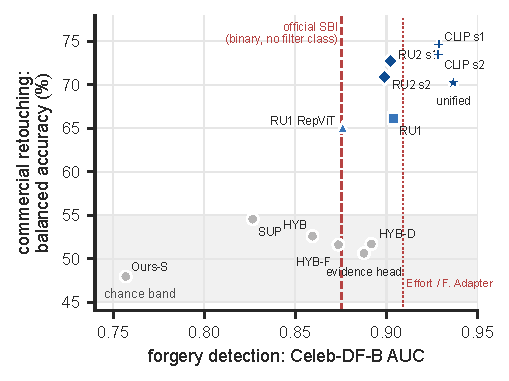
\includegraphics[width=0.5\linewidth]{fig_tradeoff}
\caption{Untreated Celeb-DF-B AUC against balanced accuracy on the unseen service, for every three-way variant. Binary
detectors have no filter class and appear as vertical lines.}
\end{figure}
\begin{table}[h]
\centering
\caption{Explanations on held-out part-level forgeries, all variants (columns as in the main paper).}
\footnotesize
\begin{adjustbox}{max width=\linewidth}\begin{tabular}{l cccc cccc cccc}
\toprule
 & \multicolumn{4}{c}{donor transplant} & \multicolumn{4}{c}{SD-1.5 inpaint} & \multicolumn{4}{c}{SDXL inpaint (unseen editor)} \\
\cmidrule(lr){2-5}\cmidrule(lr){6-9}\cmidrule(lr){10-13}
Map & IoU$_7$ & flip & ceil. & compl. & IoU$_7$ & flip & ceil. & compl. & IoU$_7$ & flip & ceil. & compl. \\
\midrule
centre prior / random region (last col.) & 0.310 & 38.6 & -- & 17.0 & 0.249 & 40.9 & -- & 17.9 & 0.255 & 40.2 & -- & 17.7 \\
\midrule
no head, Grad-CAM & 0.367 & 50.9 & 85.8 & 15.2 & 0.259 & 45.4 & 85.2 & 25.0 & 0.269 & 48.0 & 85.9 & 23.6 \\
no head, Grad-CAM++ & 0.414 & 51.7 & 85.8 & 7.2 & 0.327 & 47.8 & 85.2 & 16.7 & 0.330 & 48.8 & 85.9 & 19.1 \\
no head, Score-CAM & 0.408 & 56.5 & 85.8 & 5.9 & 0.334 & 52.4 & 85.2 & 15.4 & 0.341 & 52.4 & 85.9 & 17.1 \\
head, part edits, FF++ only & 0.723 & 84.0 & 84.7 & 0.4 & 0.752 & 82.6 & 83.2 & 0.7 & 0.746 & 82.9 & 83.8 & 0.7 \\
+ symmetric degradation & 0.723 & 86.3 & 87.1 & 0.4 & 0.719 & 82.5 & 83.7 & 2.0 & 0.728 & 83.7 & 84.4 & 1.5 \\
+ restoration-consistency loss & 0.759 & 89.4 & 90.0 & 0.4 & 0.614 & 75.2 & 79.8 & 4.4 & 0.684 & 82.5 & 84.6 & 2.6 \\
+ consistency + symmetric degradation & 0.722 & 88.4 & 89.3 & 0.7 & 0.723 & 85.2 & 86.1 & 2.4 & 0.732 & 86.1 & 86.9 & 1.8 \\
head, vendor data, no part edits (EffNet-B4) & 0.418 & 61.4 & 82.4 & 12.0 & 0.280 & 39.5 & 63.5 & 23.4 & 0.315 & 46.2 & 72.3 & 22.5 \\
head, vendor data, no part edits (CLIP) & 0.479 & 78.8 & 89.4 & 2.5 & 0.376 & 53.9 & 69.1 & 14.4 & 0.445 & 68.9 & 78.3 & 8.4 \\
\ours{}-lite (EffNet-B4) & 0.804 & 87.8 & 87.8 & 0.1 & 0.820 & 87.4 & 87.6 & 0.4 & 0.812 & 86.9 & 87.2 & 0.4 \\
\ours{} (CLIP ViT-L/14 + LoRA) & 0.832 & 91.7 & 91.9 & 0.1 & 0.845 & 91.5 & 91.6 & 0.2 & 0.827 & 90.9 & 91.2 & 0.5 \\
\bottomrule
\end{tabular}
\end{adjustbox}
\end{table}

\textbf{Measurement pitfalls.} (1) An earlier Celeb-DF-v2 set of ours (389 frames from 307 videos, filtered by
face-detector confidence) placed every published detector 3--10 AUC points above its published frame-level number; on the
standard list our scores are close to the published ones (Xception 0.718 vs.\ 0.737, EfficientNet-B4 0.750 vs.\ 0.749,
UCF 0.744 vs.\ 0.753). (2) Test crops must match the training extractor (landmark hull, 35\% margin, aspect kept); a
square $1.3\times$ crop cost our model 1.8 points. (3) Celeb-DF-B's treated videos are re-framed to portrait with
filter-tinted bars, and the landmark detector then misses 57\% of treated frames against 3\% of untreated ones; trimming
the bars restores 97\% coverage.

\textbf{Paired controls.} Without its unedited control a filter rate is a base rate: a model trained on mixed corpora
called 96.8\% of RetouchingFFHQ retouched faces \emph{filter}, and 93.9\% of their untouched originals.

\textbf{Edge model.} A RepViT-M0.9 version trained with the vendor renders keeps the commercial-retouching behaviour
(balanced 65.1\%, retouched$\to$fake 1.1\%) at 4.7\,M parameters, exports to TFLite (18\,MB, fp32) with 200/200
decisions identical to PyTorch, and runs at 9.7\,ms per image on one CPU thread. Trained with the single-operation
components it calls 55.7\% of untouched originals \emph{filter}.

\textbf{Edit-magnitude head.} A head regressing the measured quantities $q$ ranks the measured edit at Spearman
$\rho\le0.47$ for every operation on the unseen service and barely better on the training services; it is not used.

\section{Ablation over the training signal}
\begin{table}[h]
\centering
\caption{Ablation over the training signal. FF++ in-domain recall per class (\%), FA/MISS on the FF++ beautification
sets, and B1: number of binary detectors (/11 published, /12--13 with our SBI reproductions) that dominate the model.}

\footnotesize
\begin{adjustbox}{max width=\linewidth}\begin{tabular}{llccccccc}
\toprule
Variant & Fakes seen & CDFv2 & DFD & real & fake & filter & FA / MISS & B1 \\
\midrule
\ours{}-S (RepViT) & observed & 0.701 & 0.888 & 85.6 & 91.2 & 86.0 & 2.7 / 1.2 & 0/11 \\
\ours{}-SB (self-blend only) & self-blend & 0.628 & 0.879 & 95.8 & 32.2 & 36.2 & 7.4 / 22.3 & 6/12 \\
\ours{}-SUP (observed only) & observed & 0.784 & 0.912 & 80.7 & 95.0 & 88.4 & 4.9 / 0.5 & 0/13 \\
\ours{} HYB, seed 1 & both & 0.757 & 0.917 & 85.9 & 94.4 & 84.7 & 5.8 / 0.6 & 0/12 \\
\ours{} HYB, seed 2 & both & 0.770 & 0.913 & 87.6 & 92.8 & 84.3 & 4.9 / 0.7 & 0/12 \\
\ours{} HYB-F (faithful blend) & both & 0.779 & 0.900 & 82.6 & 93.8 & 84.7 & 6.1 / 0.5 & 0/13 \\
\ours{} HYB-D (+ symmetric degradation) & both & 0.807 & 0.882 & 81.6 & 91.8 & 83.7 & 5.2 / 0.8 & 0/13 \\
\ours{} HYB-PE (+ part-level edits) & both+parts & 0.810 & 0.888 & 80.7 & 90.2 & 76.8 & 8.9 / 1.6 & 0/13 \\
\ours{} HYB-PE + evidence head & both+parts & 0.819 & 0.907 & 79.0 & 90.0 & 84.0 & 7.0 / 2.1 & 0/13 \\
\ours{}-RU1 (+ vendor composites) & both+vendor & 0.826 & 0.929 & 78.0 & 93.3 & 80.7 & 8.7 / 0.4 & 0/15 \\
\textbf{\ours{}-RU2, seed 1} & both+vendor & 0.822 & 0.938 & 79.4 & 93.6 & 75.8 & 10.3 / 0.5 & 0/15 \\
\textbf{\ours{}-RU2, seed 2} & both+vendor & 0.817 & 0.934 & 80.4 & 92.9 & 76.1 & 9.9 / 0.5 & 0/15 \\
\ours{}-RU3 (cleaned components) & both+vendor & 0.832 & 0.938 & 79.8 & 93.7 & 74.9 & 10.4 / 0.6 & 0/15 \\
\ours{}-RU3 + evidence head & both+vendor & 0.824 & 0.930 & 79.9 & 94.0 & 76.4 & 10.2 / 0.3 & 0/15 \\
\textbf{\ours{}-RU3 + CLIP-L/14 LoRA, seed 1} & both+vendor & 0.878 & 0.957 & 76.7 & 94.6 & 87.9 & 5.5 / 0.2 & 0/15 \\
\textbf{\ours{}-RU3 + CLIP-L/14 LoRA, seed 2} & both+vendor & 0.883 & 0.953 & 87.2 & 92.2 & 86.9 & 4.1 / 0.5 & 0/15 \\
\ours{}-RU4 + evidence head (EffNet-B4) & both+vendor+parts & 0.848 & 0.915 & 74.2 & 93.3 & 76.4 & 11.7 / 0.5 & 0/15 \\
\textbf{\ours{}-RU4 + CLIP-L/14 LoRA (unified)} & both+vendor+parts & 0.888 & 0.948 & 78.0 & 88.9 & 89.2 & 4.0 / 0.6 & 0/15 \\
\midrule
SBI recipe, our pipeline (binary) & self-blend & 0.620 & 0.852 & -- & -- & -- & 17.5 / 28.7 & -- \\
SBI recipe, faithful blend (binary) & self-blend & 0.735 & 0.886 & -- & -- & -- & 19.3 / 20.2 & -- \\
\bottomrule
\end{tabular}
\end{adjustbox}
\end{table}

\section{Every vendor-trained variant on the unseen vendor}
\begin{table}[h]
\centering
\caption{Alibaba pairs, all vendor-trained variants (single reads). Columns as in the main paper.}
\label{tab:alipair_all}
\footnotesize
\begin{adjustbox}{max width=\linewidth}\begin{tabular}{l c cc c c c c}
\toprule
 & originals & \multicolumn{2}{c}{retouched (pooled)} & & & paired rank at level 90 & smoothing-90 \\
\cmidrule(lr){3-4}
Model & real/fake/filter & $\to$filter & $\to$fake & balanced & paired rank & eye / white / lift / smooth & $\to$fake \\
\midrule
\multicolumn{8}{l}{\textit{FF++ c23 training only (zero-shot)}} \\
three-way, RepViT-M0.9 & 0.8/2.5/96.7 & 92.6 & 6.4 & 47.9 & 48.4 & 73 / 55 / 52 / 15 & 17.7 \\
three-way, observed fakes (SUP) & 36.8/5.7/57.5 & 66.5 & 9.1 & 54.5 & 79.8 & 97 / 89 / 79 / 59 & 27.3 \\
three-way, hybrid fakes (HYB) & 33.8/16.7/49.5 & 54.6 & 22.1 & 52.6 & 69.2 & 92 / 83 / 65 / 44 & 50.2 \\
HYB, faithful blend & 28.2/22.1/49.6 & 52.8 & 28.0 & 51.6 & 65.7 & 92 / 77 / 62 / 35 & 58.4 \\
HYB + symmetric degradation & 31.7/26.3/42.0 & 45.3 & 33.6 & 51.7 & 64.3 & 89 / 76 / 63 / 35 & 63.1 \\
three-way, part edits + evidence head & 16.7/55.9/27.4 & 28.6 & 59.4 & 50.6 & 60.9 & 89 / 78 / 60 / 20 & 85.8 \\
\midrule
\multicolumn{8}{l}{\textit{Vendor-trained variants (all single Alibaba reads)}} \\
RU1 renders only (EffNet-B4, s1) & 93.4/0.8/5.8 & 38.1 & 0.6 & 66.1 & 92.8 & 99 / 85 / 95 / 100 & 0.1 \\
RU1 renders only (RepViT) & 92.8/1.4/5.9 & 36.1 & 1.1 & 65.1 & 92.6 & 96 / 89 / 93 / 100 & 0.3 \\
RU2 + components (EffNet-B4, s1) & 76.8/0.5/22.8 & 68.2 & 0.3 & 72.7 & 94.2 & 99 / 90 / 94 / 100 & 0.4 \\
RU2 + components (EffNet-B4, s2) & 66.6/0.3/33.2 & 74.9 & 0.2 & 70.8 & 94.2 & 99 / 92 / 93 / 99 & 0.4 \\
RU2 + components (RepViT) & 43.4/0.9/55.7 & 83.7 & 0.5 & 64.0 & 95.1 & 99 / 91 / 96 / 99 & 1.1 \\
RU3 cleaned components (EffNet-B4, s1) & 76.7/0.4/22.9 & 68.8 & 0.3 & 72.9 & 94.9 & 99 / 92 / 94 / 99 & 0.5 \\
RU3 + evidence head (EffNet-B4, s1) & 83.2/0.6/16.2 & 62.2 & 0.5 & 73.0 & 94.1 & 99 / 91 / 93 / 99 & 0.8 \\
RU4 + part edits (lite) (EffNet-B4, s1) & 81.0/0.4/18.6 & 63.8 & 0.3 & 72.6 & 93.8 & 99 / 91 / 93 / 99 & 0.4 \\
RU3 + evidence head, CLIP (CLIP-L/14, s1) & 77.4/0.4/22.2 & 71.4 & 0.2 & 74.6 & 93.8 & 98 / 90 / 94 / 100 & 0.2 \\
RU3 + evidence head, CLIP (CLIP-L/14, s2) & 73.0/0.3/26.7 & 73.6 & 0.2 & 73.4 & 95.1 & 99 / 94 / 96 / 100 & 0.2 \\
RU4 + part edits, CLIP (main) (CLIP-L/14, s1) & 57.9/0.3/41.9 & 82.3 & 0.1 & 70.2 & 94.8 & 98 / 94 / 95 / 100 & 0.0 \\
\bottomrule
\end{tabular}
\end{adjustbox}
\end{table}

\section{Escape per beautification preset}
\begin{figure}[h]
\centering
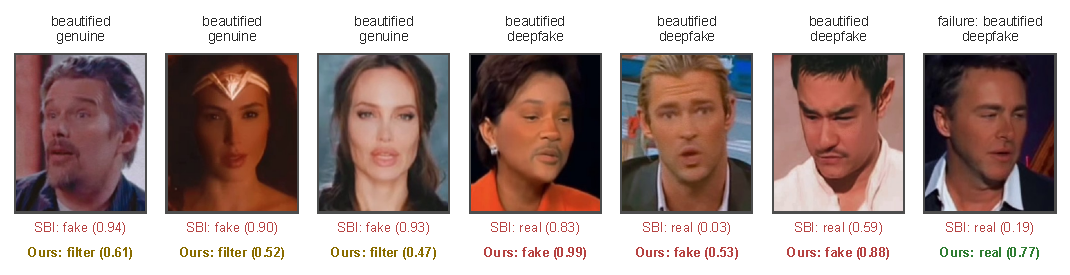
\includegraphics[width=0.95\linewidth]{fig_qual}
\caption{Celeb-DF-B examples (zero-shot): SBI's decision at its 5\%-FPR threshold on untreated genuine frames
($t=0.888$, chosen on this set) and our three-way decision. Columns 1--3: beautified genuine faces that SBI accuses and
we route to \emph{filter}; 4--6: beautified deepfakes that escape SBI and we call \emph{fake}; 7: a failure case, a
deepfake beautified with the \emph{california\_dreamin} preset that escapes us too.}

\end{figure}

\begin{table}[h]
\centering
\caption{Celeb-DF-B: change in deepfake escape rate (pp) per beautification preset, under compression alone (same
re-encoding, no filter), overall, and overall minus the compression effect.}
\footnotesize
\begin{adjustbox}{max width=0.8\linewidth}\begin{tabular}{lrrrr|r|rr}
\toprule
Detector & brown & calif. & hawaii & relax & compress & all & all$-$compr. \\
\midrule
SBI & +43.5 & +30.4 & +56.0 & +11.9 & +13.7 & +35.5 & +21.8 \\
SRM & +19.1 & +10.9 & +27.8 & +10.3 & +1.7 & +17.0 & +15.3 \\
CORE & +9.9 & +9.2 & +34.7 & +1.6 & +0.3 & +13.8 & +13.5 \\
UCF & +19.4 & +3.2 & +41.1 & -14.2 & +1.2 & +12.4 & +11.3 \\
Xception & +7.8 & +1.2 & +36.0 & -5.2 & -0.9 & +9.9 & +10.9 \\
EfficientNet-B4 & +11.9 & +1.4 & +9.0 & -9.1 & -0.1 & +3.4 & +3.4 \\
\midrule
SBI obj., our pipeline & +43.3 & +33.5 & +45.2 & +25.4 & +15.3 & +36.8 & +21.6 \\
\ours{} HYB s1 & +0.3 & +10.1 & -4.8 & +0.1 & +0.9 & +1.5 & +0.6 \\
\ours{} HYB s2 & -1.1 & +11.9 & -7.5 & +1.7 & +1.8 & +1.3 & -0.6 \\
\ours{} HYB-F & -1.2 & +5.2 & -3.6 & -0.2 & -0.3 & +0.1 & +0.3 \\
\ours{} HYB-D & -2.7 & +5.0 & -6.3 & -1.9 & -0.3 & -1.4 & -1.2 \\
\ours{}-S & -7.5 & -5.5 & -23.0 & -11.2 & -7.2 & -11.8 & -4.6 \\
\bottomrule
\end{tabular}
\end{adjustbox}
\end{table}
The grain filter (\emph{hawaii\_grain}) is the most damaging for binary detectors (+9 to +56\,pp) and lowers our escape
rate; the warm colour grading (\emph{california\_dreamin}) is our failure case (HYB +10.1 / +11.9\,pp for two seeds, RU1
+8.5\,pp), comparable to SRM and CORE.

\section{Feature space}
\begin{figure}[h]
\centering
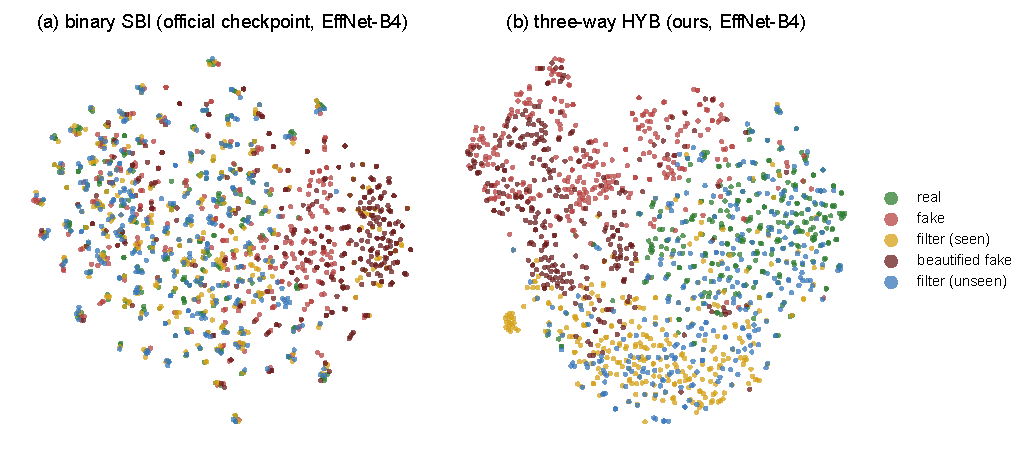
\includegraphics[width=0.75\linewidth]{fig_tsne}
\caption{t-SNE of penultimate features on the same FF++ test images (300 per group). (a) The official SBI checkpoint
separates forgeries, but beautified genuine faces are mixed with real faces, as a binary label space requires. (b) HYB forms
a filter region, and beautified forgeries stay in the fake region. Of the ten nearest labelled neighbours of a beautified
forgery, 11.7\% are genuine for SBI and 4.2\% for HYB.}
\end{figure}

\section{What the detector looks at: region restoration}
\begin{figure}[h]
\centering
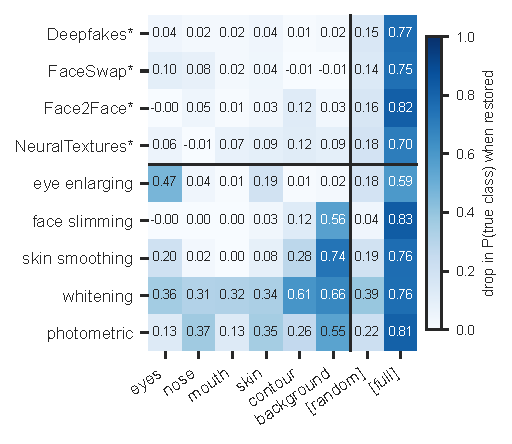
\includegraphics[width=0.55\linewidth]{fig_restore}
\caption{Region restoration on correctly classified FF++ test images: drop in $P(\text{true class})$ when one facial region
is restored to its unedited pixels. [random]: area-matched patch at a random location; [full]: whole image restored.
*Forgeries use the real frame of the same video, resized to the fake crop (approximate alignment).}
\end{figure}
Grad-CAM peaks at the face centre for every class, and occlusion with a constant fill injects a blending-like seam that
itself pushes the model toward \emph{fake}. Restoring a region to its pixel-aligned original is a cleaner test. Eye
enlargement is carried by the eyes (0.47 vs 0.18 for a random patch of equal area); face slimming by the pixels the warp
displaces around the jaw. Skin smoothing is carried mostly by the \emph{background} (0.74) rather than the skin (0.08):
our scripted smoothing acts on the whole frame, and the detector uses the smoothed background. For forgeries no single
region carries the decision (every region $\le$0.12), while restoring the whole frame removes it (0.70--0.82).

\section{Unseen photometric filters}
On 11 photometric filters never seen in training, applied to FF++ test frames, HYB routes 51.8\% of frames to \emph{filter}
against 7.4\% for the unedited frames (paired excess 44.7--45.5\,pp) and calls 9.5\% of them \emph{fake}; the RepViT model's
excess is ${\approx}$52\,pp with 4.6\% fake calls. RU2 keeps a paired excess of 31--34\,pp.

\section{Evidence head: detection, per-source recall, robustness, cost, output}
\begin{table}[h]
\centering
\caption{Detection with and without the evidence head, same backbone and recipe; 61.5k part edits in the fake pool (the
first consistency-loss variant saw 43.4k). Celeb-DF-B: untreated AUC and \% of untreated genuine frames called fake.}
\footnotesize
\begin{adjustbox}{max width=\linewidth}\begin{tabular}{lcccccccc}
\toprule
 & \multicolumn{2}{c}{CDFv2} & \multicolumn{2}{c}{DFD} & & & & Celeb-DF-B \\
\cmidrule(lr){2-3}\cmidrule(lr){4-5}
Variant & frame & video & frame & video & FF++ real/fake/filter & FA / MISS & B1 & AUC / accus. \\
\midrule
\ours{}-PE (no head) & 0.810 & 0.871 & 0.888 & 0.853 & 80.7/90.2/76.8 & 8.9 / 1.6 & 0/13 & 0.879 / 56.0 \\
\textbf{+ evidence head (ours)} & 0.819 & 0.878 & 0.907 & 0.866 & 79.0/90.0/84.0 & 7.0 / 2.1 & 0/13 & 0.888 / 60.6 \\
+ evidence head + symmetric degradation & 0.817 & -- & 0.896 & -- & 82.8/81.3/79.7 & 5.5 / 4.8 & 0/13 & 0.894 / 17.9 \\
+ consistency loss (43k edits) & 0.794 & -- & 0.905 & -- & 83.1/89.1/87.2 & 3.2 / 2.6 & 0/13 & 0.870 / 50.7 \\
+ consistency + symmetric degradation & 0.781 & -- & 0.877 & -- & 84.7/80.8/79.6 & 6.2 / 5.1 & 0/13 & 0.875 / 15.1 \\
\bottomrule
\end{tabular}
\end{adjustbox}
\end{table}
\begin{table}[h]
\centering
\caption{FF++ test routing of the evidence-head model by source (\% of frames sent to each class; bold: correct class).}
\footnotesize
\begin{adjustbox}{max width=0.6\linewidth}\begin{tabular}{llrrrr}
\toprule
Class & Source & $n$ & $\to$real & $\to$fake & $\to$filter \\
\midrule
real & genuine & 1316 & \textbf{79.2} & 13.8 & 7.1 \\
fake & Deepfakes & 1327 & 1.0 & \textbf{98.9} & 0.2 \\
fake & Face2Face & 1326 & 4.0 & \textbf{94.8} & 1.2 \\
fake & FaceSwap & 1323 & 7.6 & \textbf{92.3} & 0.2 \\
fake & NeuralTextures & 1328 & 22.6 & \textbf{73.9} & 3.5 \\
filter & smoothing & 156 & 0.0 & 7.1 & \textbf{92.9} \\
filter & whitening & 149 & 3.4 & 8.1 & \textbf{88.6} \\
filter & eye enlarging & 152 & 49.3 & 13.8 & \textbf{36.8} \\
filter & face slimming & 150 & 16.7 & 4.7 & \textbf{78.7} \\
filter & photometric (14) & 709 & 2.0 & 5.8 & \textbf{92.2} \\
\bottomrule
\end{tabular}
\end{adjustbox}
\end{table}
\begin{figure}[h]
\centering
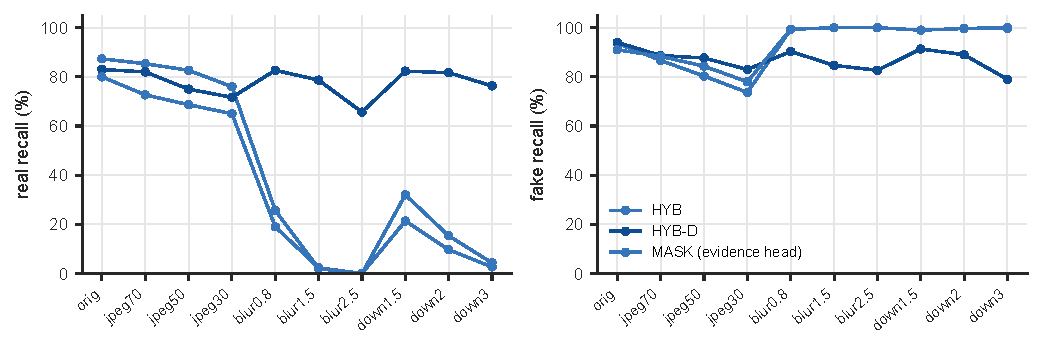
\includegraphics[width=0.8\linewidth]{fig_robust_MASK}
\caption{Recall of genuine (left) and forged (right) FF++ test frames under JPEG re-compression, Gaussian blur and
downscaling (300 frames each). Models trained without symmetric degradation call almost every blurred genuine frame fake.}
\end{figure}
\begin{table}[h]
\centering
\caption{Single-image cost (batch 1, PyTorch fp32; CPU: desktop, GPU: RTX 6000 Ada), mean of 50 runs.}
\footnotesize
\begin{adjustbox}{max width=0.7\linewidth}\begin{tabular}{lrrrr}
\toprule
Model & Params (M) & Input & CPU (ms) & GPU (ms) \\
\midrule
RepViT-M0.9 (ours-S) & 4.7 & 224 & 28.3 & 8.3 \\
EfficientNet-B4 (HYB) & 17.6 & 380 & 55.0 & 10.7 \\
EfficientNet-B4 + evidence head (MASK) & 17.6 & 380 & 62.1 & 10.3 \\
\bottomrule
\end{tabular}
\end{adjustbox}
\end{table}
NeuralTextures, whose edits are confined to the mouth, is the weakest forgery method (73.9\%); eye enlargement at our
scripted strengths is recognised at 37\%. Under blur or downscaling the models without symmetric degradation collapse on
genuine frames (2\% at $\sigma=1.5$) while HYB-D keeps 66--83\%. The head adds 0.01\,M parameters and 7\,ms on CPU.

\section{System output of \ours{}}
\begin{figure}[h]
\centering
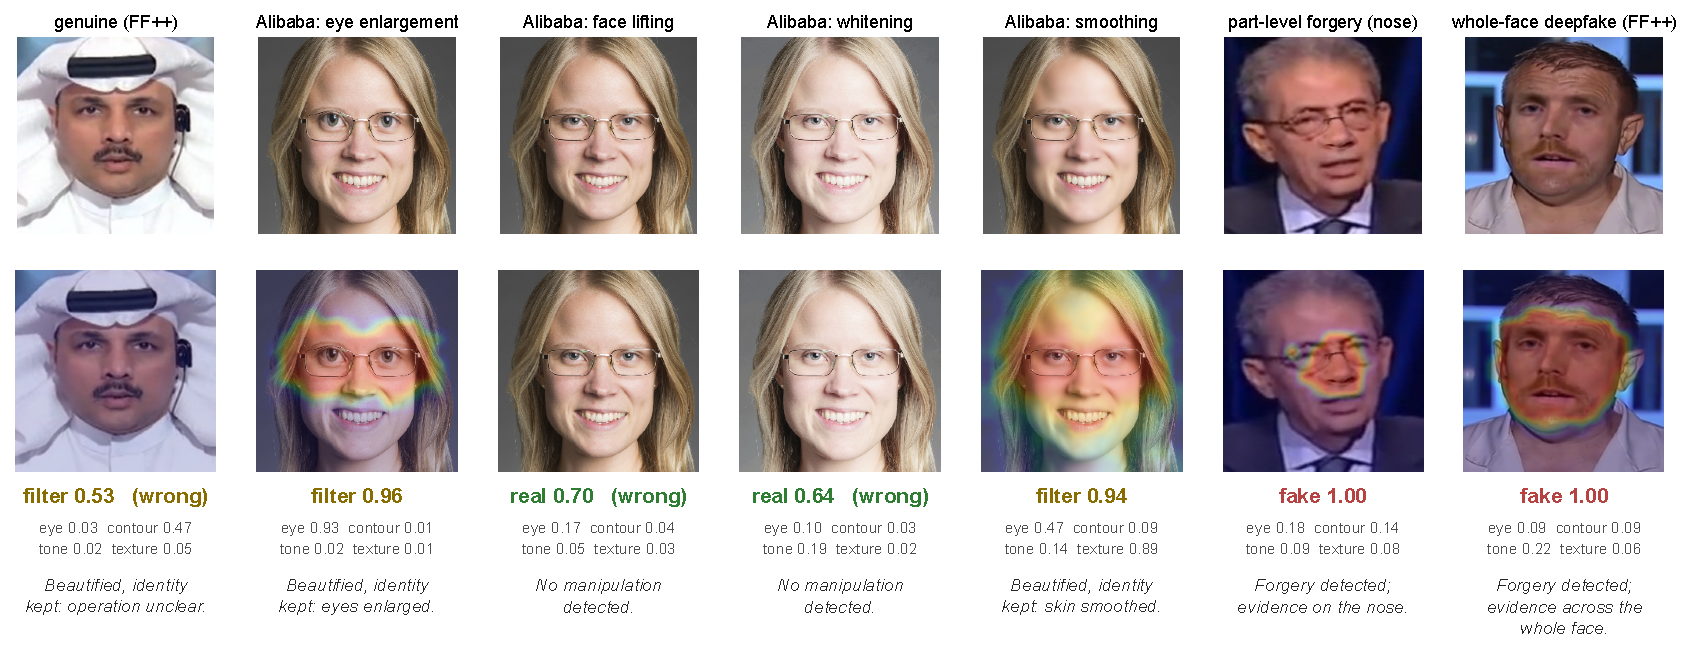
\includegraphics[width=\linewidth]{fig_system_output}
\caption{Output of \ours{} on examples fixed in advance: one FF++ genuine frame, the four Alibaba renders of one FFHQ face
at level 90, a held-out part-level forgery and an FF++ Deepfakes frame. Per image: the three-way decision and its
probability, the presence score of each operation, the evidence map, and a template sentence. The sentence names the
operations with presence $\ge 0.5$ (filter) or the facial part with the highest mean evidence (fake; ``whole face'' when
eyes, nose and mouth all exceed 0.5). No language model is involved. Three of the seven are wrong: lifting and whitening
are missed and the genuine frame is sent to \emph{filter}.}
\end{figure}
The facial part is named by the mean evidence inside each landmark region. On held-out part-level forgeries (every fourth
item, detected ones) this names the edited part in 99.0\%, 98.5\% and 97.7\% of cases for the donor, SD and SDXL editors.
Naming it by the share of the top-12\% evidence region that falls on each part, as in an earlier version, names it in only
8--12\%, because the skin region is large; the map itself is unchanged. Operation names are reliable on the training
services' held-out faces for whitening and smoothing (presence recall 0.79--0.99) and weaker for eye enlargement and face
reshaping (0.50--0.80); on the unseen service they drop to 0.21 (eyes), 0.35 (reshaping), 0.57 (whitening) and 0.96
(smoothing). On 379 fixed test images the template produces 14 distinct sentences: one for \emph{real}, four for
\emph{fake} and nine for \emph{filter}. The edit-magnitude estimates are not shown because they did not pass validation
(Sec.~S1).

\end{document}
